% -*- compile-command: "rubber -d Fibonacci.tex" -*-
\documentclass{article}

\usepackage{hyperref}
\usepackage{url}
\usepackage{amsmath}

\usepackage[outputdir=diagrams, extension=pgf, backend=pgf, input]{diagrams-latex}
\usepackage{pgf}

\usepackage{graphicx}
\graphicspath{{images/}}

%%%%%%%%%%%%%%%%%%%%%%%%%%%%%%%%%%%%%%%%%%%%%%%%%%%%%%%%%%%%

\title{Fibonacci numbers}
\author{Brent Yorgey, \href{http://www.mathlesstraveled.com}{\texttt{mathlesstraveled.com}} \\ \raisebox{-0.4em}{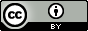
\includegraphics[width=44px]{../CC-BY.png}} \href{http://creativecommons.org/licenses/by/4.0/}{\texttt{creativecommons.org/licenses/by/4.0/}}}

\begin{document}

\maketitle

\fontsize{16}{20}\selectfont

The \emph{Fibonacci numbers} are defined by
\begin{align*}
  F_0 &= 0 \\
  F_1 &= 1 \\
  F_n &= F_{n-1} + F_{n-2} & (n > 1)
\end{align*}

The first 17 Fibonacci numbers are therefore \[
  0,1,1,2,3,5,8,13,21,34,55,89,144,233,377,610,987. \]

\begin{enumerate}
  \item What is the next Fibonacci number?  \vspace{1in}
  \item If $F_{28} = 317811$ and $F_{29} = 514229$, what is $F_{27}$?
  \item Backwards Fibonacci numbers
  \item Things to count: pavements, Fibonacci trees
\item\end{enumerate}

\end{document}
